\documentclass{beamer}
\usetheme{Madrid}

\usepackage{cmap}
\usepackage[T2A]{fontenc}
\usepackage[russian,english]{babel}
\usepackage[utf8]{inputenc}
\usepackage{amsmath, amssymb}
\usepackage{minted}
\usepackage{hologo}

\usepackage{algorithm2e}
\usepackage{algorithmic}
\usepackage{float}

\usepackage{cancel}
\usepackage{ulem}

% \newtcbox{\mybox}{blank, on line, opacitytext=0.5}

\title[Ускорение обучения языковых моделей]{Методы предобработки текстовых данных для ускорения обучения языковых моделей с помощью обучения по плану}

\author[Сурков М.К.]{Сурков Максим Константинович\\
 	{\footnotesize Научный руководитель: Ямщиков Иван Павлович}
}
\institute[НИУ ВШЭ СПБ]{Санкт-Петербургская школа физико-математических и компьютерных наук \\ НИУ ВШЭ СПБ}
\date{20 апреля 2021 г.}

\begin{document}

\frame{\titlepage}

\begin{frame}
	\frametitle{Мотивация. Применения}
	\begin{columns}
		\column{0.5\textwidth}
		\begin{itemize}
			\item социальные сети
			\item голосовые помощники
			\item переводчики
			\item чат-боты
		\end{itemize}
		\column{0.5\textwidth}
		
\includegraphics[scale=0.2]{nlp_real_life.png}
	\end{columns}
	\noindent\makebox[\linewidth]{\rule{\paperwidth}{0.4pt}}
	\begin{columns}
		\column{0.5\textwidth}
		\begin{itemize}
			\item классификация
			\item машинный перевод
			\item вопросно-ответные системы
		\end{itemize}
		\column{0.5\textwidth}
		\begin{itemize}
			\item небольшие языковые модели
			\item GPT-3
			\begin{itemize}
				\item очень большая модель
			\end{itemize}
			\item {\bf BERT}
			\begin{itemize}
				\item высокое качество
			\end{itemize}
		\end{itemize}
	\end{columns}
\end{frame}

\begin{frame}
	\frametitle{Мотивация. Обучение языковой модели}
	
\includegraphics[scale=0.4]{pre_training_fine_tuning.png}
	\begin{columns}
		\column{0.5\textwidth}
			\begin{itemize}
				\item требуемое время: от 1-2 дней до {\bf 1-2 недель}
				\item мировой рекорд: 47 минут с использованием {\bf 1472} GPU

				\begin{table}
					\begin{tabular}{l|c}
						Корпус данных & Размер \\
						\hline\hline
						Wikipedia & 3-600M \\
						BookCorpus & 74M\\
					\end{tabular}
				\end{table}
			\end{itemize}
		\column{0.5\textwidth}
			\begin{itemize}
				\item требуемое время: 1-2 дня

				\begin{table}
					\begin{tabular}{l|c}
						Корпус данных & Размер \\
						\hline\hline
						HND & 600k-2M \\
						s140 & 1.6M \\
						IWSLT & 200-230k \\
						QQP & 364k \\
						MNLI & 393k \\
					\end{tabular}
				\end{table}
			\end{itemize}
	\end{columns}
	\noindent\makebox[\linewidth]{\rule{\paperwidth}{0.4pt}}
	\begin{itemize}
		\item {\bf долго} обучать
		\item нужно обрабатывать {\bf большие} объемы данных
	\end{itemize}
\end{frame}

\begin{frame}
	\frametitle{Обучение по плану. Определение}
	\begin{columns}
		\column{0.5\textwidth}
		\begin{enumerate}
			\item сортируем данные по сложности (длина)
			\item в течение $T$ шагов (рассмотрим $t$-й шаг)
			\begin{itemize}
				\item вычисляем $c(t) \in [0, 1]$
				\item формируем пакет данных маленького размера из множества $c(t)$ {\bf легких} примеров
				\item шаг обучения
			\end{itemize}
		\end{enumerate}
		\column{0.5\textwidth}
		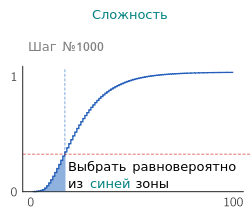
\includegraphics[scale=0.8]{acl19_algo.png}
	\end{columns}
	\let\thefootnote\relax\footnotetext{Platanios et al., 2019}
\end{frame}

\begin{frame}
	\frametitle{Метод сравнения алгоритмов обучения}
	\begin{columns}
		\column{0.5\textwidth}
		\begin{enumerate}
			\item фиксируем: корпус данных, модель, семплер
			\item обучаем модель
			\item фиксируем достаточно большой порог (точность, функция потерь)
			\item сравниваем графики
			\item или сравниваем среднее число шагов, необходимое для достижения данного порога
		\end{enumerate}
		\column{0.5\textwidth}
		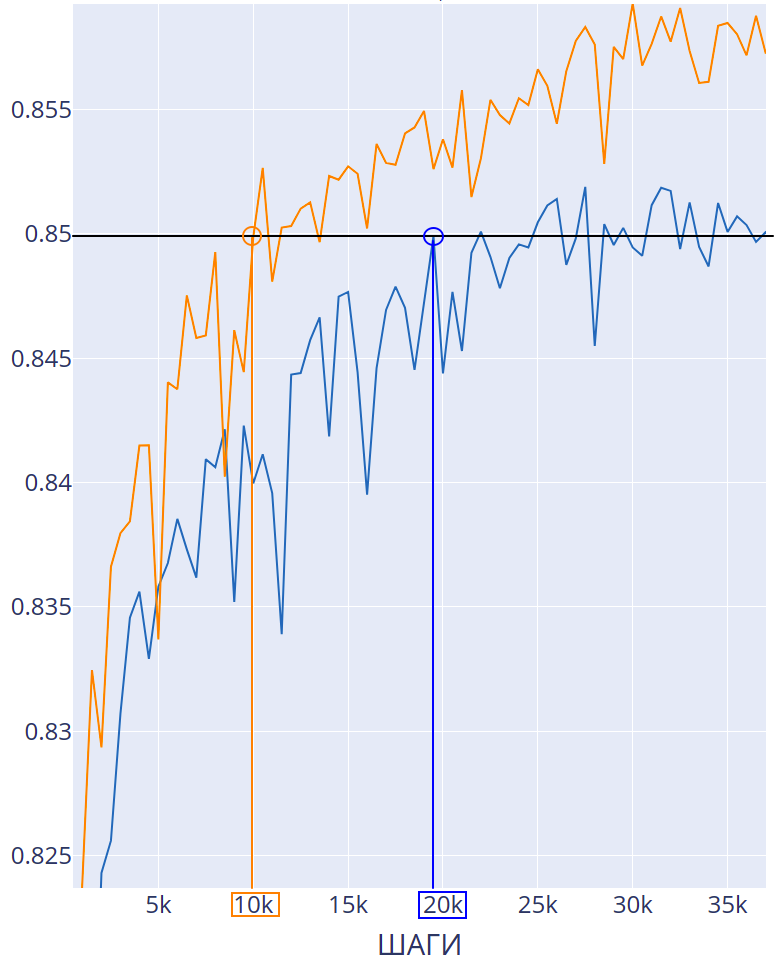
\includegraphics[scale=0.25]{compare}
	\end{columns}
\end{frame}

\begin{frame}
	\frametitle{Поле исследований}
	\begin{table}
		\begin{tabular}{l|cccc}
			метрика & классификация & перевод & предобучение & NLU\footnote[1]{вопросно-ответная система} \\
			\hline
			длина & & $\checkmark$ & & \\
			{\it языковая}\footnote[2]{Sluis et al. (2010) показали слабую корреляцию с реальной сложностью текста} & & & & \\
			энтропия & & & & \\
			модельная & & & & $\checkmark$ \\
			частота слов & & $\checkmark$ & & \\
			правдоподобие & & $\checkmark$ & & \\
			\hline
			? & & & & \\
			\hline
		\end{tabular}
	\end{table}
	\begin{itemize}
		\item не изучено влияние обучения по плану на задачах классификации и предобучения
		\item покрыто узкое множество метрик (длина - лучшая метрика на данный момент)
		\item нет универсального решения
	\end{itemize}
\end{frame}

\begin{frame}
	\frametitle{Цель и задачи}
	{\bf Цель:} ускорить обучение языковой модели BERT с помощью обучения с расписанием за счет метрики оценки сложности текстовых данных на задачах предобучения и классификации
	
	{\bf Задачи:}
	\begin{enumerate}
		\item Предложить метрики оценки сложности текста
		\item Реализовать производительные алгоритмы вычисления предложенных метрик на больших наборах данных
		\item Сравнить найденные метрики с существующими метриками оценки сложности текста
		\item Исследовать влияние найденных метрик на скорость обучения языковой модели BERT
	\end{enumerate}
\end{frame}

\begin{frame}
	\frametitle{Поиск метрик}
	\begin{enumerate}
		\item  база
		\begin{itemize}
			\item {\bf длина}, вероятность правдоподобия (Platanios et al., 2019)
			\item самое редкое слово в предложении (Xuan Zhang et al., 2018)
		\end{itemize}
		\item информационный поиск
		\begin{itemize}
			\item {\bf tf-idf}
		\end{itemize}
		\item {\bf теория информации} (Nihat Ay et al., 2006)
		\begin{itemize}
			\item EE, TSE
				\[
				T=(t_1, t_2, \ldots, t_{i-1},t_i,\ldots, t_n)
				\]
				\[
				\downarrow
				\]
				\[
				\xi=(\xi^1_{t_1},\xi^2_{t_2},\ldots,\xi^{i-1}_{t_{i-1}},\xi^i_{t_i},\ldots,\xi^n_{t_n})
				\]
				\[
				t_i\rightarrow \xi^i_{t_i} =: \mu_i - \text{бинарная случайная величина}
				\]
		\end{itemize}
		\item модельная
		\begin{itemize}
			\item MLM-loss
		\end{itemize}
	\end{enumerate}
\end{frame}

\begin{frame}
	\frametitle{Вычисление метрик}
	\begin{itemize}
		\item EE, TSE
			\begin{itemize}
				\item сложные математическая формулы
				\item $\mathcal{O^*}(2^n), \mathcal{O}(n^2)$ -- несравнимо долго $\rightarrow$ алгоритм за $\mathcal{O}(n)$
			\end{itemize}
		\item максимальный частотный ранг
			\begin{enumerate}
				\item вычисляем частоту каждого слова
				\item присваиваем каждому слову позицию в массиве, отсортированном по убыванию частоты
				\item сложность предложения -- максимальный ранг по всем словам в предложении
			\end{enumerate}
		\item правдоподобие
			\[
				L(T) = -\sum\limits_{i=1}^{n}\log f(t_i), \text{ где } f(x) \text{ -- частота слова}
			\]
		\item MLM-loss
			\begin{itemize}
				\item учим BERT на задаче MLM (Пример: "Привет, как [МАСКА]?"), оптимизируя кросс-энтропию
				\item сложность = значение кросс-энтропии на данном тексте
			\end{itemize}
	\end{itemize}
\end{frame}

\begin{frame}
	\frametitle{Вычисление метрик}
	\begin{itemize}
		\item статистики
			\begin{enumerate}
				\item длина $\rightarrow$ число текстов с такой длиной
				\item $(i, x_i) \rightarrow$ число текстов, где $t_i = x_i$ 
				\item $(x_i)\rightarrow$ число текстов, где $x_i$ является последним токеном
				\item $(i, x_{i-1}, x_i) \rightarrow$ число текстов, где на $(i-1)$-й позиции стоит $x_{i-1}$, а на $i$-й позиции стоит $x_i$
				\item $x_i \rightarrow$ число текстов, в которых есть $x_i$
			\end{enumerate}
		\item сбор статистик в параллельном режиме (разделение по данным)
		\item вычисление MLM-loss требует GPU
	\end{itemize}
	\noindent\makebox[\linewidth]{\rule{\paperwidth}{0.4pt}}
	Итого:
	\begin{itemize}
		\item предложены подходы, покрывающие широкое множество метрик
		\item предложены алгоритмы, вычисляющие метрики за пренебрежимо маленькое время (по сравнению со временем обучения)
	\end{itemize}
\end{frame}

\begin{frame}
	\frametitle{Сравнение метрик. Предобучение}
	\begin{columns}
		\column{0.5\textwidth}
			\begin{itemize}
				\item Обучение по плану сильно проигрывает базовому решению
				\item метрики имеют порядок вне зависимости от семплера
				\begin{enumerate}
					\item {\bf максимальный ранг слова}
					\item TF-IDF
					\item EE
					\item TSE
					\item правдоподобие
					\item длина
				\end{enumerate}
				\item длина проигрывает остальным метрикам
				\item семплеры имеют порядок вне зависимости от метрики
			\end{itemize}
		\column{0.5\textwidth}
			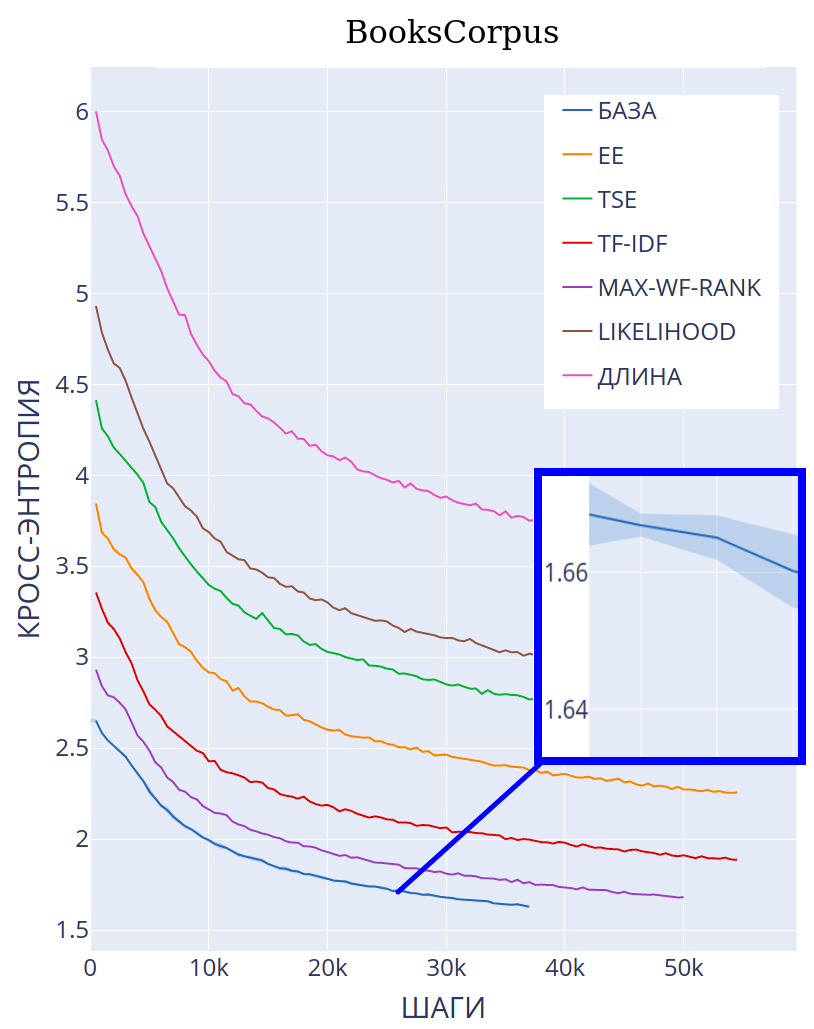
\includegraphics[scale=0.28]{BookCorpus_results}
	\end{columns}
\end{frame}

\begin{frame}
	\frametitle{Сравнение метрик. Классификация}
	$\max\Delta \le 3k$
	\begin{table}
		\begin{tabular}{l|ccccc}
			Корпус данных & \multicolumn{4}{c}{sentiment140 (85.5\%)}\\
			\hline
			семплер & CB & DB & Hyp & SS & SM\\
			\hline
			длина (86.2\%) & 112.5k & 20k & 19k & - & -\\
			TF-IDF (86.7\%) & 115.5k & 21.5k & 19.5k & 16.5k & 22k\\
			TSE (86.8\%) & 95.5k & 16.5k & 20.5k & 21.5k & 18k\\
			EE (86.7\%) & 59k & 16.5k & 23k & 20k & 19k\\
			max wf rk (86.7\%) & 70k & 18.5k & 19.5k & 17k & 19k\\
			правдоподобие (86.7\%) & 112k & 17.5k & 21.5k & 17.5k & 21.5k\\
			MLM-loss (86.1\%) & 59.5k & 21k & 23.5k & ? & ?\\
			\hline
			база (87\%) & \multicolumn{4}{c}{18k}
		\end{tabular}
	\end{table}
	\begin{itemize}
		\item нет статистически значимой разницы в метриках (искл.: длина, MLM-loss)
		\item длина ухудшает качество модели
		\item влияние семплера много больше влияния метрики на скорость обучения
	\end{itemize}
\end{frame}

\begin{frame}
	\frametitle{Влияние метрик на скорость обучения}
	\begin{itemize}
		\item любая конфигурация обучения по плану проигрывает стандартному алгоритму обучения
		\item влияние токенизатора: нет
		\item влияние гиперпараметров обучения: нет
		\item влияние опыта предобученной модели на обучение по плану: нет
		\begin{itemize}
			\item замена предобученного BERT-base на случайно инициализированный не приводит к выигрышу обучения по плану
		\end{itemize}
		\item BERT переобучается на длину: нет (семплеры SS, SM)
		\item итоговое распределение датасета неравномерное: нет (DB, Hyp)
	\end{itemize}
\end{frame}

\begin{frame}
	\frametitle{Результаты}
	\begin{enumerate}
		\item Предложен широкий спектр метрик оценки сложности текста
		\begin{itemize}
			\item метрики TSE и EE адаптированы под задачу обработки языка
		\end{itemize}
		\item Реализованы алгоритмы подсчета метрик на больших объемах данных
		\item Проведено сравнительное исследование метрик
			\begin{itemize}
				\item длина проигрывает всем
				\item предобучение: есть строгий порядок (Wikipedia, BookCorpus)
				\item классификация: нет значимых отличий (s140, HND)
			\end{itemize}
		\begin{itemize}
			\item показано, что влияние метрики зависит от семплера
		\end{itemize}
		\item поведение метрик зависит от задачи $\Rightarrow$ не удалось найти универсального решения
		\item Не удалось добиться существенного ускорения относительно базового подхода на задачах предобучения и классификации
	\end{enumerate}
\end{frame}

\appendix

\begin{frame}[label=supplemental,noframenumbering]
	\frametitle{Дополнительно: Вычисление EE}
	\[
	EE(X) = \left[\sum\limits_{v\in V}H(X_{V\backslash\{v\}})\right] - (n - 1)H(X_V) = 
	\]
	\[
	\left[\sum\limits_{i=1}^{n}H(\mu_1,\ldots,\mu_{i-1},\mu_{i+1},\ldots,\mu_n)\right] - (n - 1)H(\mu)
	\]
	\begin{itemize}
		\item $\mathcal{O}(n^2)$
		\item $\mathcal{O}(n)$
		\[
		\sum\limits_{i=1}^{n}H(\mu_1,\ldots,\mu_{i-1},\mu_{i+1},\ldots,\mu_n) =\]
		\[ = \sum\limits_{i=1}^{n}H(\mu) - H(\mu_i|\mu_{i-1}) - H(\mu_{i+1}|\mu_i) + H(\mu_{i+1})\]
		\[
		EE(X) = \sum\limits_{i=2}^{n}H(\mu_i) - H(\mu_i|\mu_{i-1})= \sum\limits_{i=2}^{n}I(\mu_{i-1}\colon\mu_i)
		\]
	\end{itemize}
\end{frame}

\begin{frame}[label=supplemental,noframenumbering]
	\frametitle{Дополнительно: Вычисление TSE}
	\[
	\sum\limits_{k=1}^{n-1}\frac{k}{n}C^{(k)}(X_V)
	\]
	\[
	C^{(k)}(X_V) = \frac{n}{k\binom{n}{k}}\sum\limits_{A\subseteq V,|A|=k}H(X_A) - H(X_V) =
	\]
	\[
	= \frac{n}{k}\left[\frac{1}{\binom{n}{k}}\sum\limits_{A\subseteq V,|A|=k}H(X_A)\right] - H(X_V)
	\]
\end{frame}

\begin{frame}[label=supplemental,noframenumbering]
	\frametitle{Дополнительно: Вычисление TSE}
	\[
	\frac{1}{\binom{n}{k}}\sum\limits_{A\subseteq V,|A|=k}H(X_A) =
	\frac{1}{\binom{n}{k}}\sum\limits_{1 \le i_1 < i_2 < \ldots < i_k \le n}H(\mu_{i_1}, \mu_{i_2}, \ldots, \mu_{i_k})
	\]
	\begin{enumerate}
		\item $\mathcal{O^*}(2^n)$
		\item $\mathcal{O}(n^2)$ - динамическое программирование
		\item $\mathcal{O}(n)$
		\[
		\sum\limits_{i=1}^{n}A_iH(\mu_i) + \sum\limits_{i=2}^{n}B_iH(\mu_i|\mu_{i-1})
		\]
		\[
		A_i = 
		\begin{cases}
		\binom{n-2}{k-1}/\binom{n}{k}=\frac{k(n-k)}{n(n-1)},& i > 1 \\
		\binom{n-1}{k-1}/\binom{n}{k}=\frac k n,& i = 1
		\end{cases}
		\]
		\[
		B_i = \frac{\binom{n-2}{k-2}}{\binom{n}{k}} = \frac{k(k-1)}{n(n-1)}
		\]
	\end{enumerate}
\end{frame}

\begin{frame}
	\frametitle{Результаты. классификация. HND}
	
	Корпус данных: Hyperpartisan News Detection
	
	$\max\Delta \le 3k$
	\begin{table}
		\begin{tabular}{l|ccccc}
			Корпус данных & \multicolumn{4}{c}{HND (92.9\%)}\\
			\hline
			семплер & CB & DB & Hyp & SS & SM\\
			\hline
			length (93.7\%) & 55k & 23k & 22.5k & - & -\\
			TF-IDF (93.5\%) & $\infty$ & 19.5k & 24k & 23.5k & 33k\\
			TSE (93.8\%) & 56.5k & 21k & 23k & 22k & 31k\\
			EE (93.8\%) & 71.5k & 25.5k & 22.5k & 19.5k & 32.5k\\
			max wf rk (93.6\%) & $\infty$ & 22k & 20.5k & 22.5k & 39k\\
			правдоподобие (93.8\%) & $\infty$ & 20k & 24k & 20k & 30k\\
			\hline
			база (93.8\%) & \multicolumn{4}{c}{22k}
		\end{tabular}
	\end{table}
\end{frame}

\end{document}